\chapter{Ejemplos de fractales}

\section{Copo de Koch}

\subsection{Construcción}

\noindent Comenzamos con un segmento de longitud $1$.

\begin{figure}[H]
    \centering
    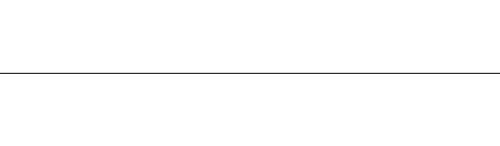
\includegraphics[width=0.5\textwidth]{figures/kock-curve-iteration-0.png}
    \caption{Iteración cero de la curva de Koch.}
    \label{fig:koch-curve-iteration-0}
\end{figure}

\noindent En la primera iteración, dividimos el segmento en tres partes iguales y reemplazamos la parte central por dos segmentos de la misma longitud, formando un ángulo de $60^\circ$. \cite{eswiki:copo-koch}

\begin{figure}[H]
    \centering
    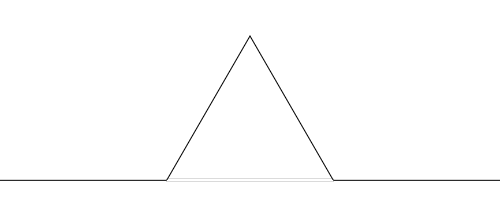
\includegraphics[width=0.5\textwidth]{figures/kock-curve-iteration-1.png}
    \caption{Primera iteración de la curva de Koch.}
    \label{fig:koch-curve-iteration-1}
\end{figure}

\noindent Para siguientes iteraciones, repetimos el mismo proceso para todos los segmentos. \cite{eswiki:copo-koch}

\begin{figure}[H]
    \centering
    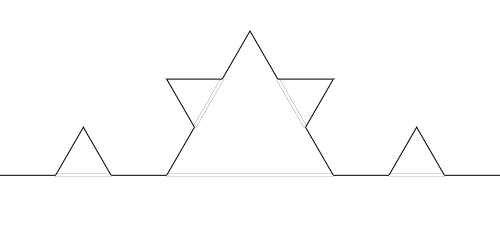
\includegraphics[width=0.5\textwidth]{figures/kock-curve-iteration-2.png}
    \caption{Segunda iteración de la curva de Koch.}
    \label{fig:koch-curve-iteration-2}
\end{figure}

\subsection{Propiedades}

\noindent El copo de Kock es un objeto autosimilar, con autosimilitud exacta. \cite{youtube-2022}

\begin{figure}[H]
\centering
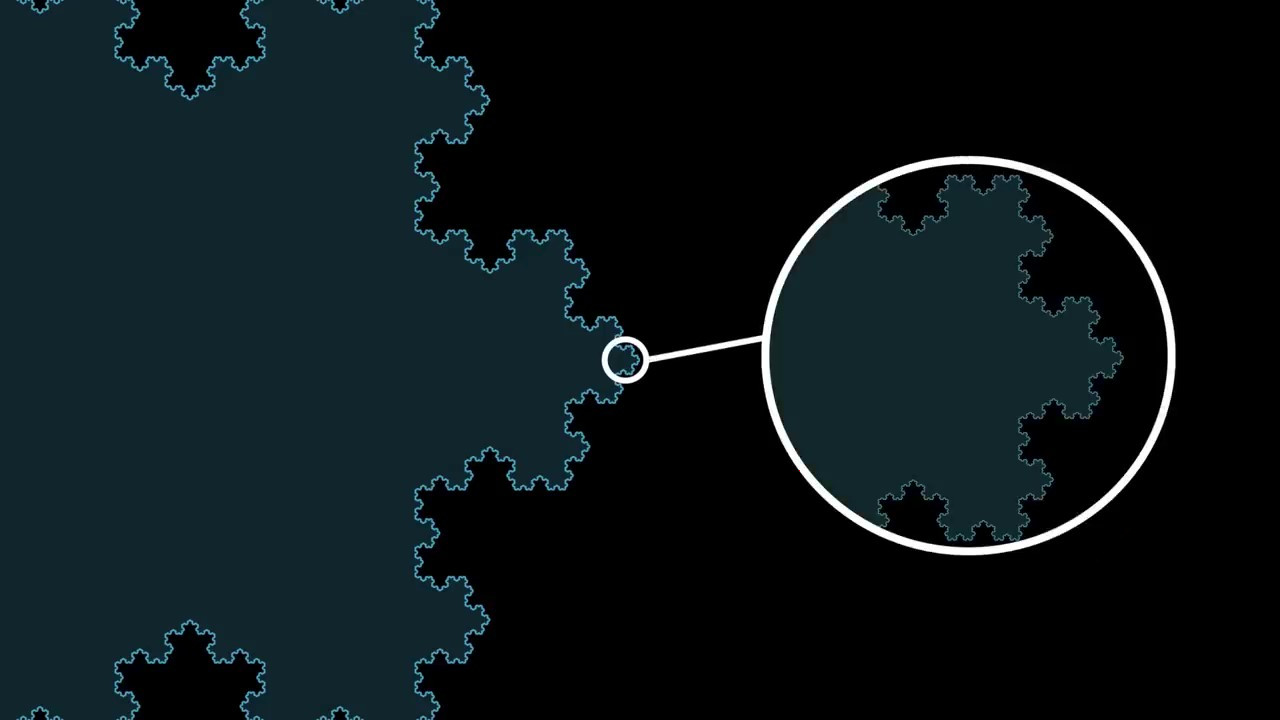
\includegraphics[width=0.5\textwidth]{figures/kock-snowflake-self-similarity.jpg}
\caption{Autosilitud exacta del copo de Koch.}
\label{fig:koch-snowflake-self-similarity}
\cite{youtube-2022}
\end{figure}

\noindent La dimensión fractal del copo de Koch es $\frac{\log 4}{\log 3} \approx 1.26186$ \cite{eswiki:copo-koch}\\

\begin{figure}[H]
    \centering
    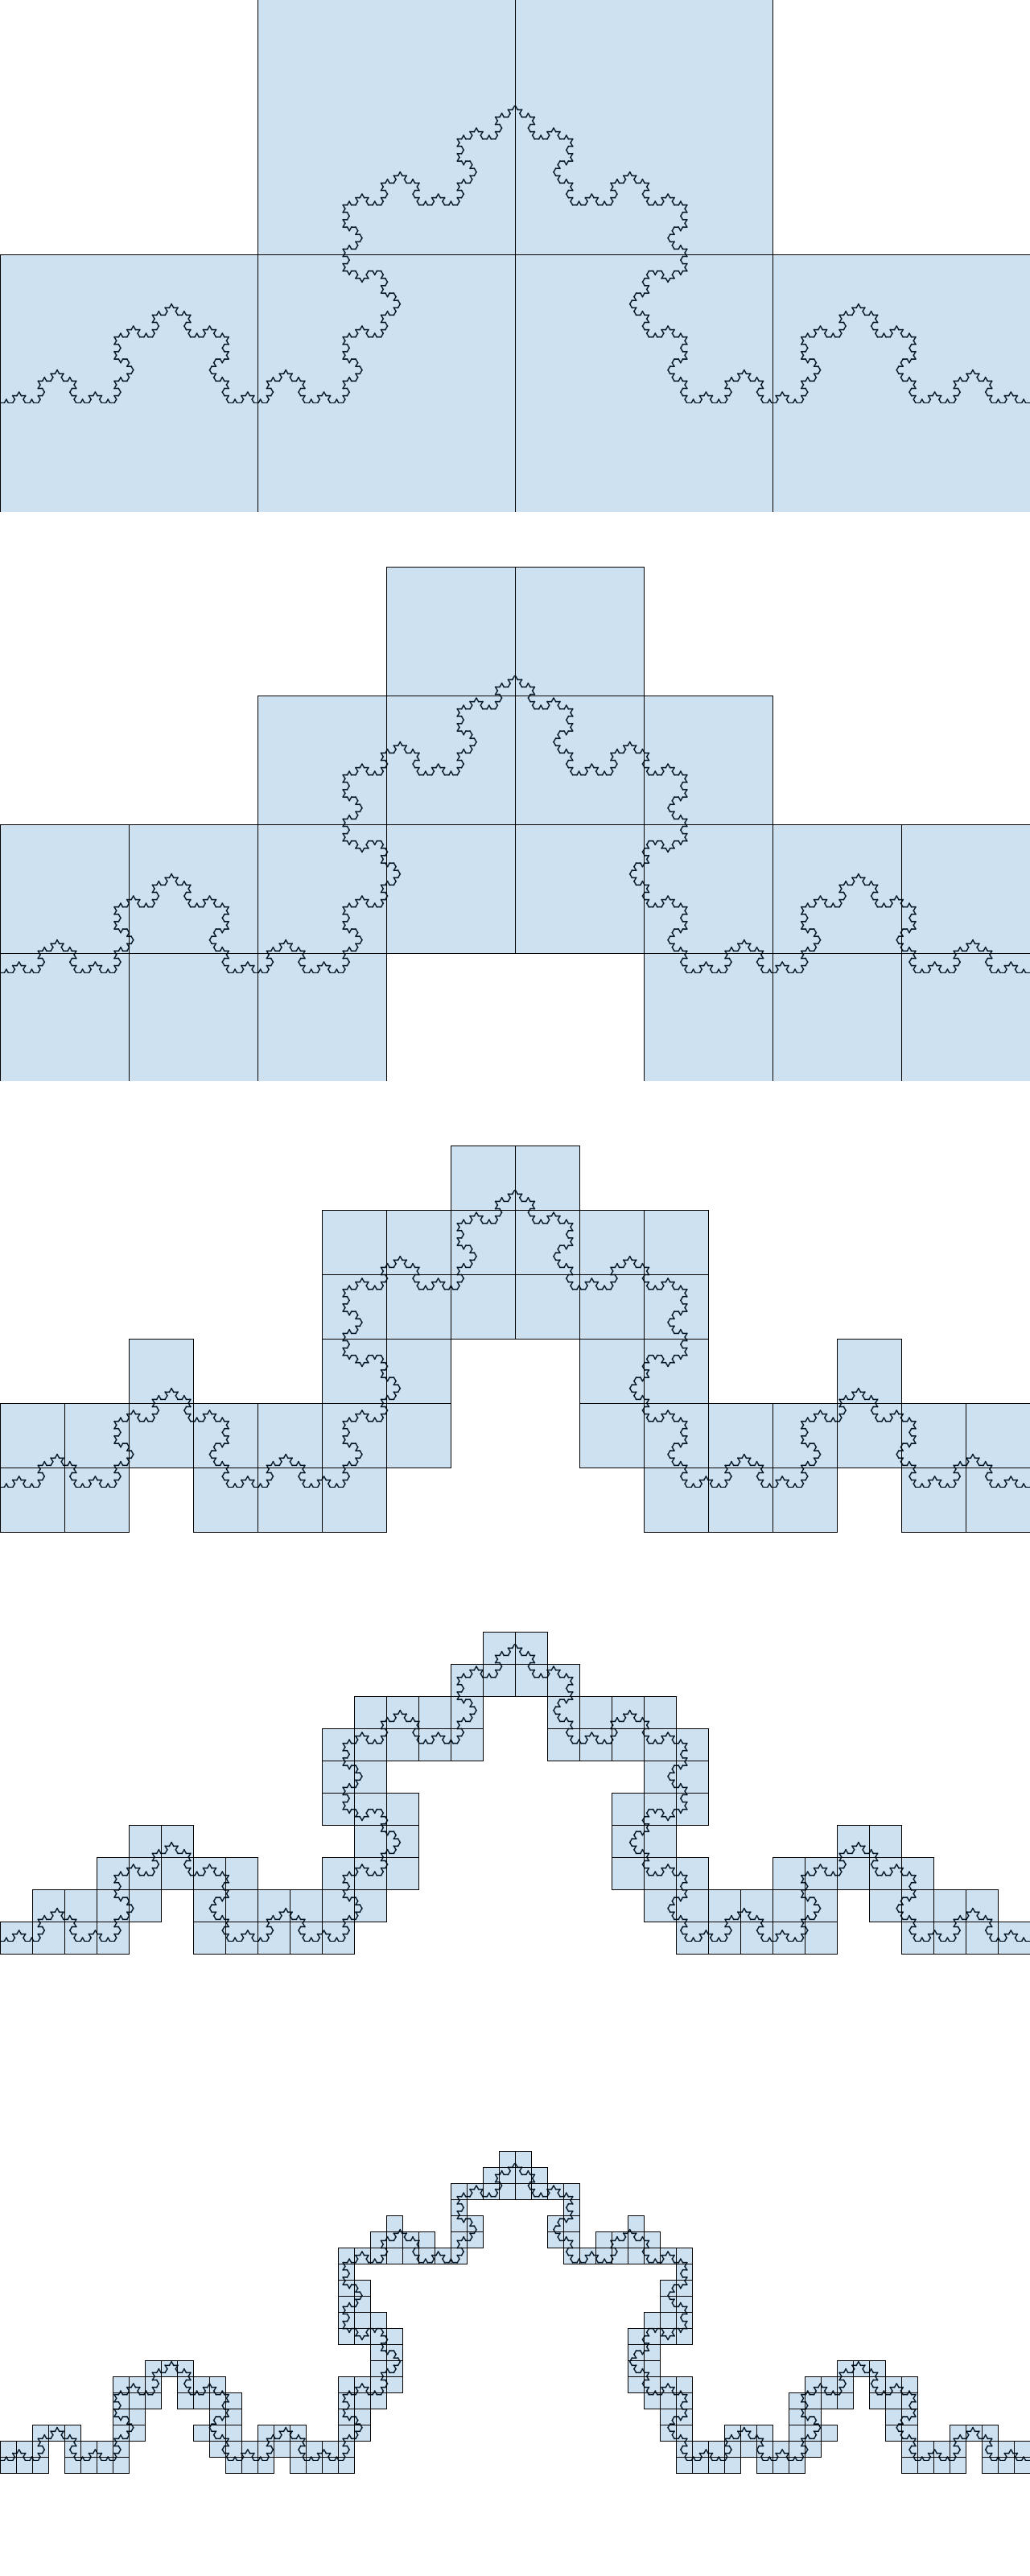
\includegraphics[width=0.5\textwidth]{figures/box-counting-koch-snowflake.png}
    \caption{Box counting del copo de Koch.}
    \label{fig:box-counting-koch-snowflake}
\end{figure}

\begin{theorem}
    El copo de Kock tiene longitud infinita, pero área finita. \cite{youtube-2022}
\end{theorem}

\begin{proof}
    \noindent Primero definamos $N(n)$ como el número de lados del polígono en la iteración $n$ y $L(n)$ como la longitud de cada lado del polígono en la iteración $n$.\\

    \noindent En el inicio, $N(0) = 3$ y $L(0) = 3$\\
    
    \begin{figure}[H]
        \centering
        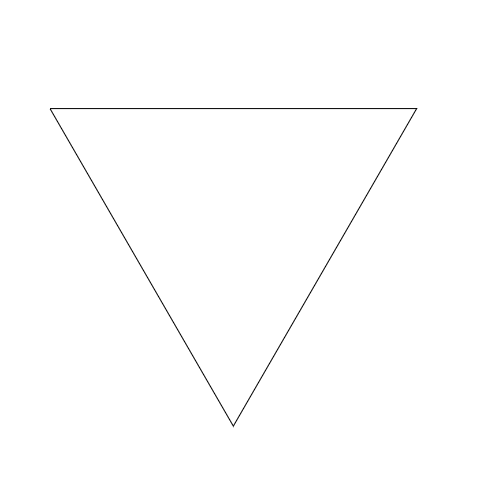
\includegraphics[width=0.5\textwidth]{figures/koch-snowflake-iteration-0.png}
        \caption{Iteración cero del copo de Koch.}
        \label{fig:koch-snowflake-iteration-0}
    \end{figure}
    
    \noindent En la primera iteración, $N(1) = 3 \cdot 4$ y $L(1) = 3 \cdot \frac{4}{3}$\\
    
    \begin{figure}[H]
        \centering
        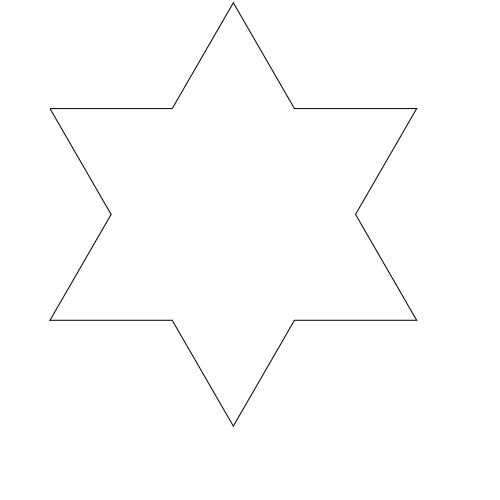
\includegraphics[width=0.5\textwidth]{figures/koch-snowflake-iteration-1.png}
        \caption{Primera iteración del copo de Koch.}
        \label{fig:koch-snowflake-iteration-1}
    \end{figure}
    
    \noindent En la segunda iteración, $N(2) = 3 \cdot 4^2$ y $L(2) = 3 \cdot \left(\frac{4}{3}\right)^2$\\
    
    \begin{figure}[H]
        \centering
        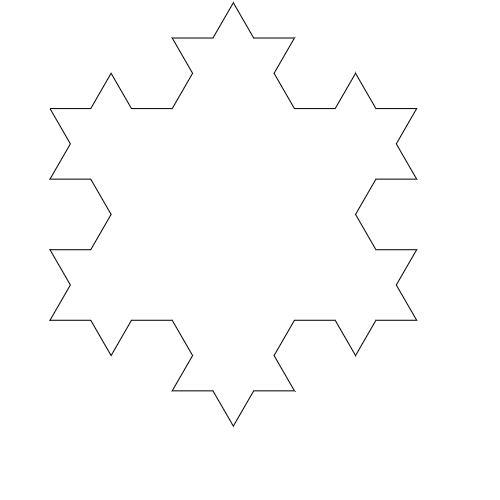
\includegraphics[width=0.5\textwidth]{figures/koch-snowflake-iteration-2.png}
        \caption{Segunda iteración del copo de Koch.}
        \label{fig:koch-snowflake-iteration-2}
    \end{figure}
    
    \noindent En la iteración $n$, $N(n) = 3 \cdot 4^n$ y $L(n) = 3 \cdot \left(\frac{4}{3}\right)^n$\\
    
    \begin{figure}[H]
        \centering
        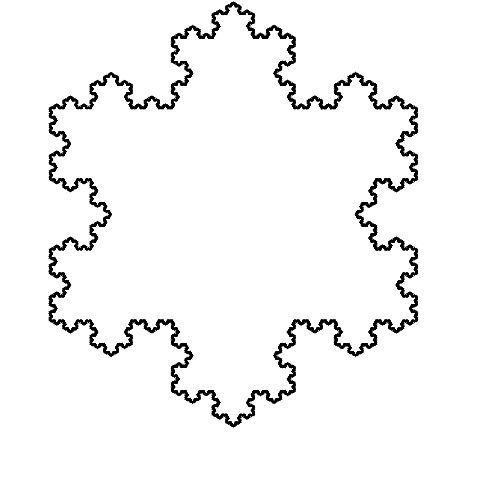
\includegraphics[width=0.5\textwidth]{figures/koch-snowflake-iteration-n.png}
        \caption{Iteración $n$ del copo de Koch.}
        \label{fig:koch-snowflake-iteration-n}
    \end{figure}
    
    \noindent Viendo esto es facil ver que cuando $n \to \infty$, $L(n) \to \infty$\\
    
    \begin{equation}
        \lim_{n \rightarrow \infty}L(n) = \lim_{n \rightarrow \infty} 3 \cdot \left(\frac{4}{3}\right)^n = \infty
    \end{equation}
    
    \noindent El área claramente es finita ya que podemos contener el copo en un círculo. \cite{youtube-2022}\\
    
    \begin{figure}[H]
        \centering
        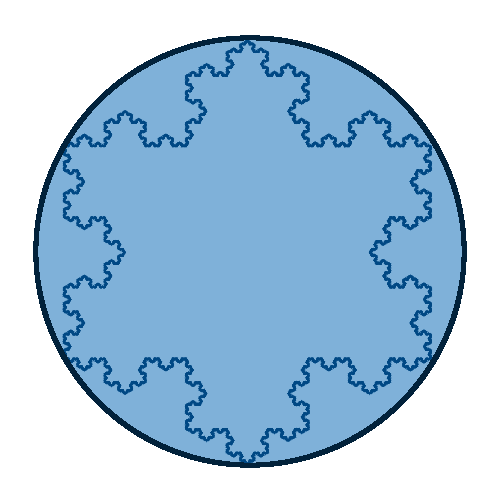
\includegraphics[width=0.5\textwidth]{figures/koch-snowflake-circle.png}
        \caption{Copo de Koch dentro de un círculo.}
        \label{fig:koch-snowflake-circle}
    \end{figure}
\end{proof}

\section{Set de Mandelbrot}

\noindent El set de Mandelbrot es un conjunto bidimensional que con una definición muy simple produce estructuras complejas y hermosas.\\

\noindent Aunque el nombre esté relacionado con el matemático Benoît Mandelbrot, el set fue definido por primera vez en 1978 por Robert W. Brooks y Peter Matelski. \cite{Wikipedia_Mandelbrot}

\begin{figure}[H]
    \centering
    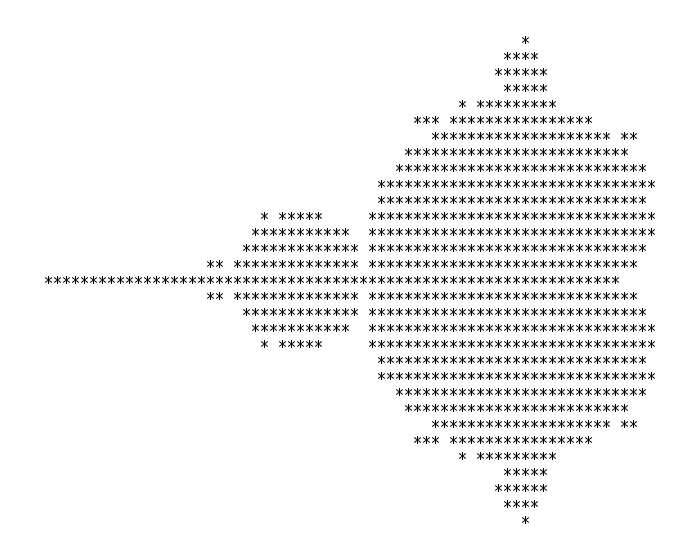
\includegraphics[width=0.5\textwidth]{figures/mandelbrot-set-first-picture.png}
    \caption{Primera imagen publicada del set de Mandelbrot, por Robert W. Brooks y Peter Matelski.}
    \label{fig:mandelbrot-set-first-picture}
\end{figure}

\subsection{Construcción}

\begin{definition}
    El conjunto de Mandelbrot es el conjunto de números complejos $c$ para los cuales el método iterativo definido por $z_0 = 0$ y $z_{n+1} = z_n^2 + c$ no tiende al infinito, es decir, no es divergente.\cite{Medina_2011}
\end{definition}

\noindent En las representaciones gráficas se suele mostrar en negro los puntos que no divergen (los que pertencen al conjunto). El resto de puntos se colorean en función de cuantas iteraciones tardan en exceder un límite en el que ya se supone que divergen.\\

\noindent Para ver si excede el límite podemos usar el módulo del número complejo, el cual representa la distancia de este con el origen. Por ejemplo, si nuestro fractal está definido en $[-1,1] \times [-1,1]$, entonces diremos que $mod(z)>2 \implies \text{divergente}$.
Si completa las $1000$ iteraciones, asumimos que converge y lo pintamos de negro.\\

\begin{lstlisting}[language=Python]
def mandelbrot(x, y):
    c = complex(x, y)
    z = 0

    for i in range(1, 1000):
        if abs(z) > 2:
            return rgb_conv(i)
        z = z * z + c
    return (0, 0, 0)
\end{lstlisting}

\subsection{Propiedades}

\begin{theorem}
    El conjunto de Mandelbrot es compacto. \cite{Wikipedia_Mandelbrot}
\end{theorem}

\begin{lemma}
    Un subconjunto cerrado de un compacto es compacto.
\end{lemma}

\begin{lemma}
    Un círculo es compacto.
\end{lemma}

\begin{lemma}
    El conjunto de Mandelbrot es cerrado.
\end{lemma}

\begin{proof}
    Como el conjunto de Mandelbrot es un conjunto cerrado y es un subconjunto del círculo de radio $2$, entonces también es compacto.
\end{proof}

\begin{theorem}
    El conjunto de Mandelbrot es conexo. \cite{Wikipedia_Mandelbrot}
\end{theorem}

\noindent En 2001, Jeremy Kahn demostró que efectivamente el conjunto es conexo. 

\section{Fractales basados en simulaciones físicas}

\noindent Algunos fractales pueden aparecer como resultado de simulaciones físicas. Esto se debe a que estas simulaciones a menudo producen mucho caos (un pequeño cambio en las condiciones inciales produce resultados dispares), y los fractales están muy relacionados con la teoría del caos.\cite{youtube-2016}\\

\subsection{Fractal a partir de imanes}

\noindent Podemos generar un fractal a partir de tres imanes y una bola de acero colgada de un hilo. Cada pixel representará la posición incial de la bola y el color (rojo, amarillo o azul) representará el imán en el que termina.\\

\begin{figure}[H]
    \centering
    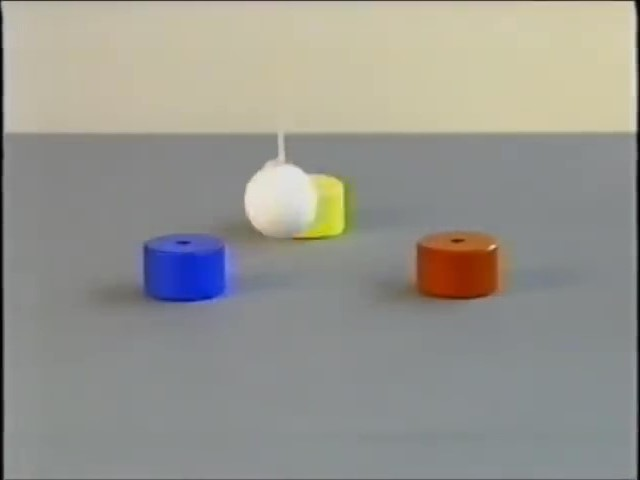
\includegraphics[width=0.5\textwidth]{figures/magnets.jpg}
    \caption{Tres imanes y una bola de acero.}
    \label{fig:magnets}
\end{figure}

\begin{figure}[H]
    \centering
    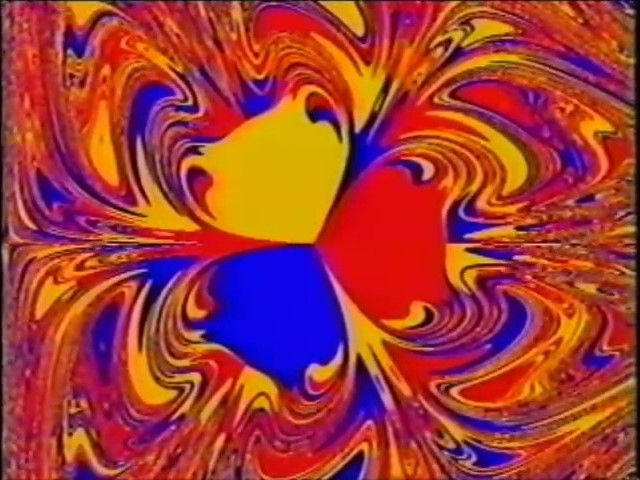
\includegraphics[width=0.5\textwidth]{figures/magnet-fractal.jpg}
    \caption{Fractal generado a partir de tres imanes y una bola de acero.}
    \label{fig:magnets-fractal}
\end{figure}

\noindent En cada línea hay otra de diferente color, por lo que podemos seguir haciendo zoom a priori de forma infinita.\\

\begin{figure}[H]
    \centering
    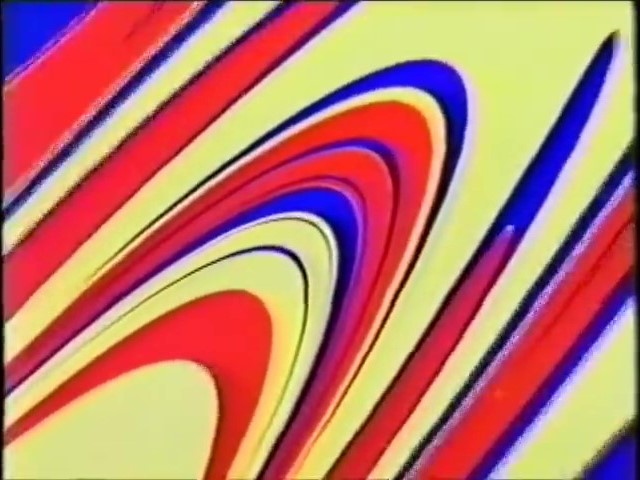
\includegraphics[width=0.5\textwidth]{figures/magnet-fractal-zoom.jpg}
    \caption{Zoom en el fractal generado a partir de tres imanes y una bola de acero.}
    \label{fig:magnets-fractal-zoom}
\end{figure}

\subsection{Fractal a partir de pelotas rebotando en una función}

\noindent Podemos generar un fractal a partir de una función y una pelota que rebota en ella \cite{balls}. Cada pixel representará la posición incial de la pelota y el color del pixel será cuantos botes tarda en llegar al lado contrario del que empezó. Si la pelota rebota más de $1000$ veces suponemos que se queda en bucle y pintamos el pixel de negro\\ 

\noindent Hemos utilizado la función $f(x)= x^4 - x^2$, pero se podrían usar otras funciones.

\begin{figure}[H]
    \centering
    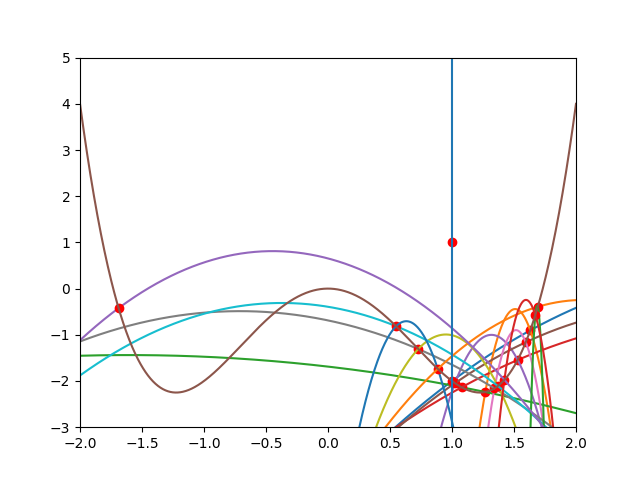
\includegraphics[width=0.7\textwidth]{figures/ball.png}
    \caption{Visualizción de los botes de la pelota $(1,1)$}
    \label{fig:ball-(1,1)}
\end{figure}

\begin{figure}[H]
    \centering
    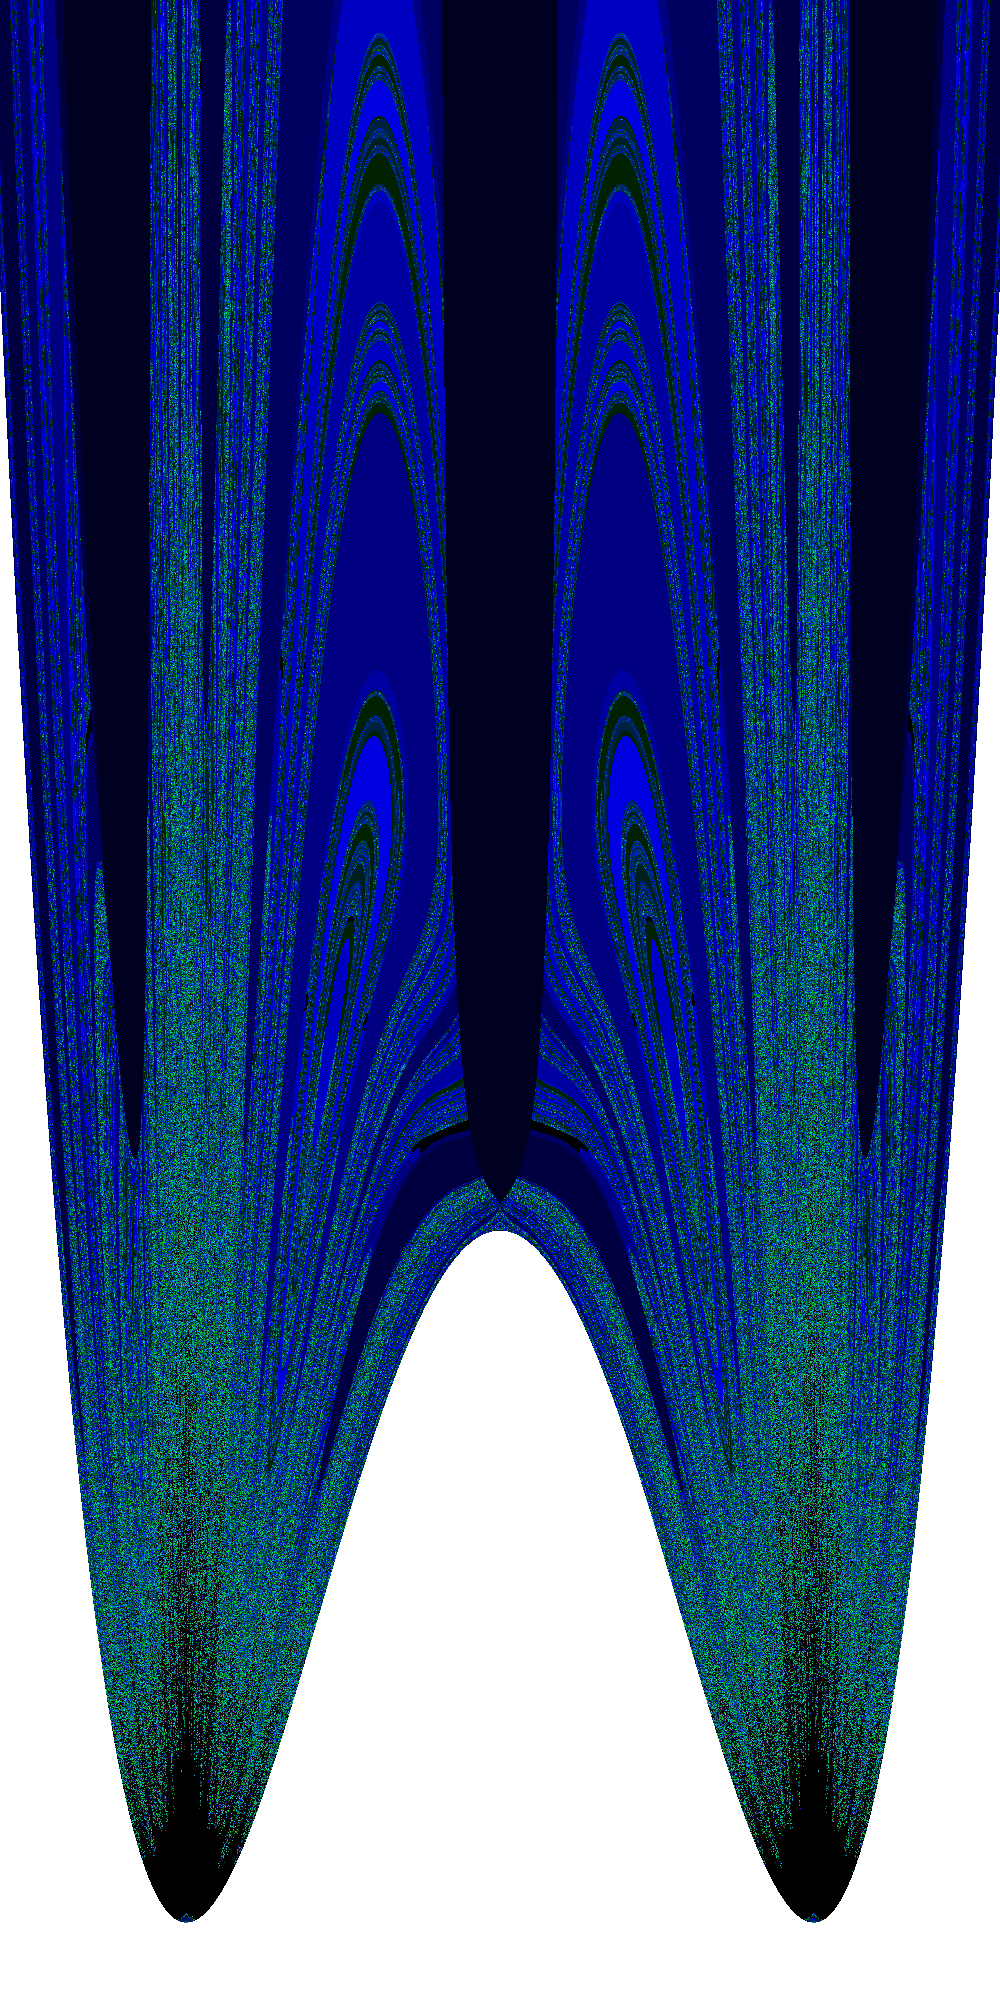
\includegraphics[width=0.7\textwidth]{figures/bouncing-ball-fractal.png}
    \caption{Fractal generado a partir de $f(x) = x^4 - x^2$ y una pelota que rebota en ella.}
    \label{fig:ball-fractal}
\end{figure}

\noindent En las elipses del objeto se puede ver una autosimilitud aproximada. Se parece un poco al fractal magnético.
\begin{figure}[H]
    \centering
    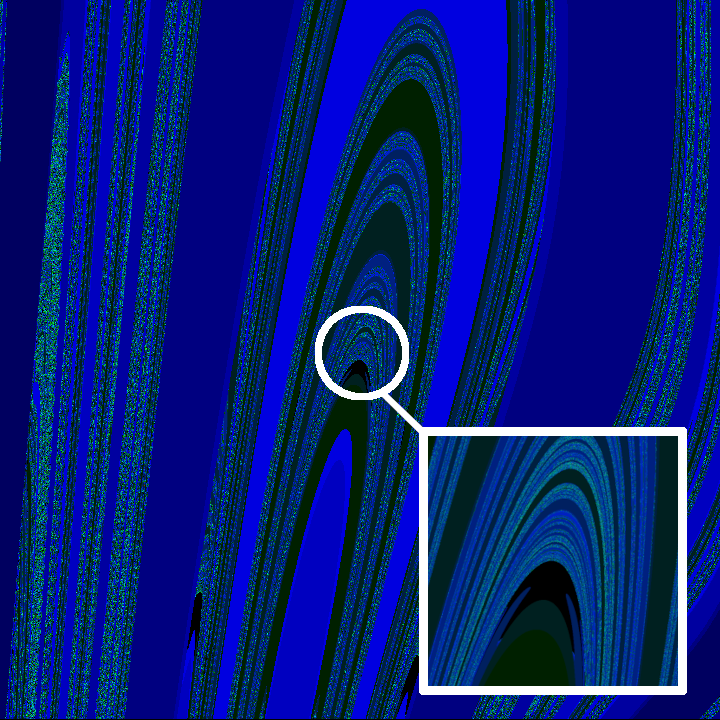
\includegraphics[width=0.7\textwidth]{figures/bouncing-ball-fractal-zoom-1.png}
    \caption{Zoom a una de las elipses del fractal generado a partir de $f(x) = x^4 - x^2$ y una pelota que rebota en ella.}
    \label{fig:ball-fractal-zoom}
\end{figure}

\noindent Hay otras formas interesantes, aunque no tienen autosimilitud.

\begin{figure}[H]
    \centering
    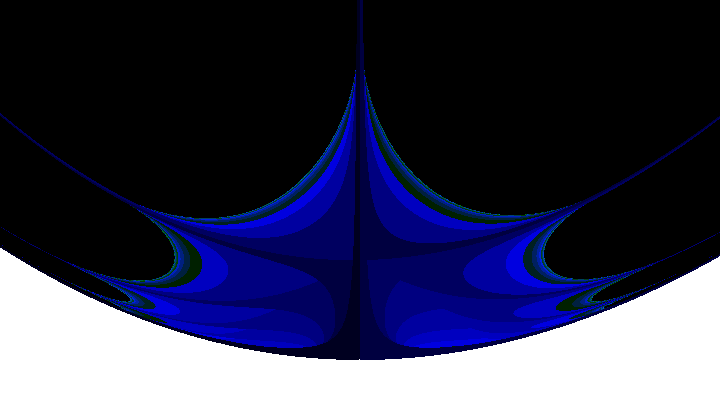
\includegraphics[width=0.7\textwidth]{figures/bouncing-ball-fractal-zoom-2.png}
    \caption{Zoom a una de las patas del fractal generado a partir de $f(x) = x^4 - x^2$ y una pelota que rebota en ella.}
    \label{fig:ball-fractal-zoom-2}
\end{figure}

\section{Fractales de papel}

\noindent Los fractales de papel son una forma creativa de crear fractales con nuestras propias manos. A través de pliegues y cortes precisos en el papel podemos manufacturarlos.\\

\begin{figure}[H]
    \centering
    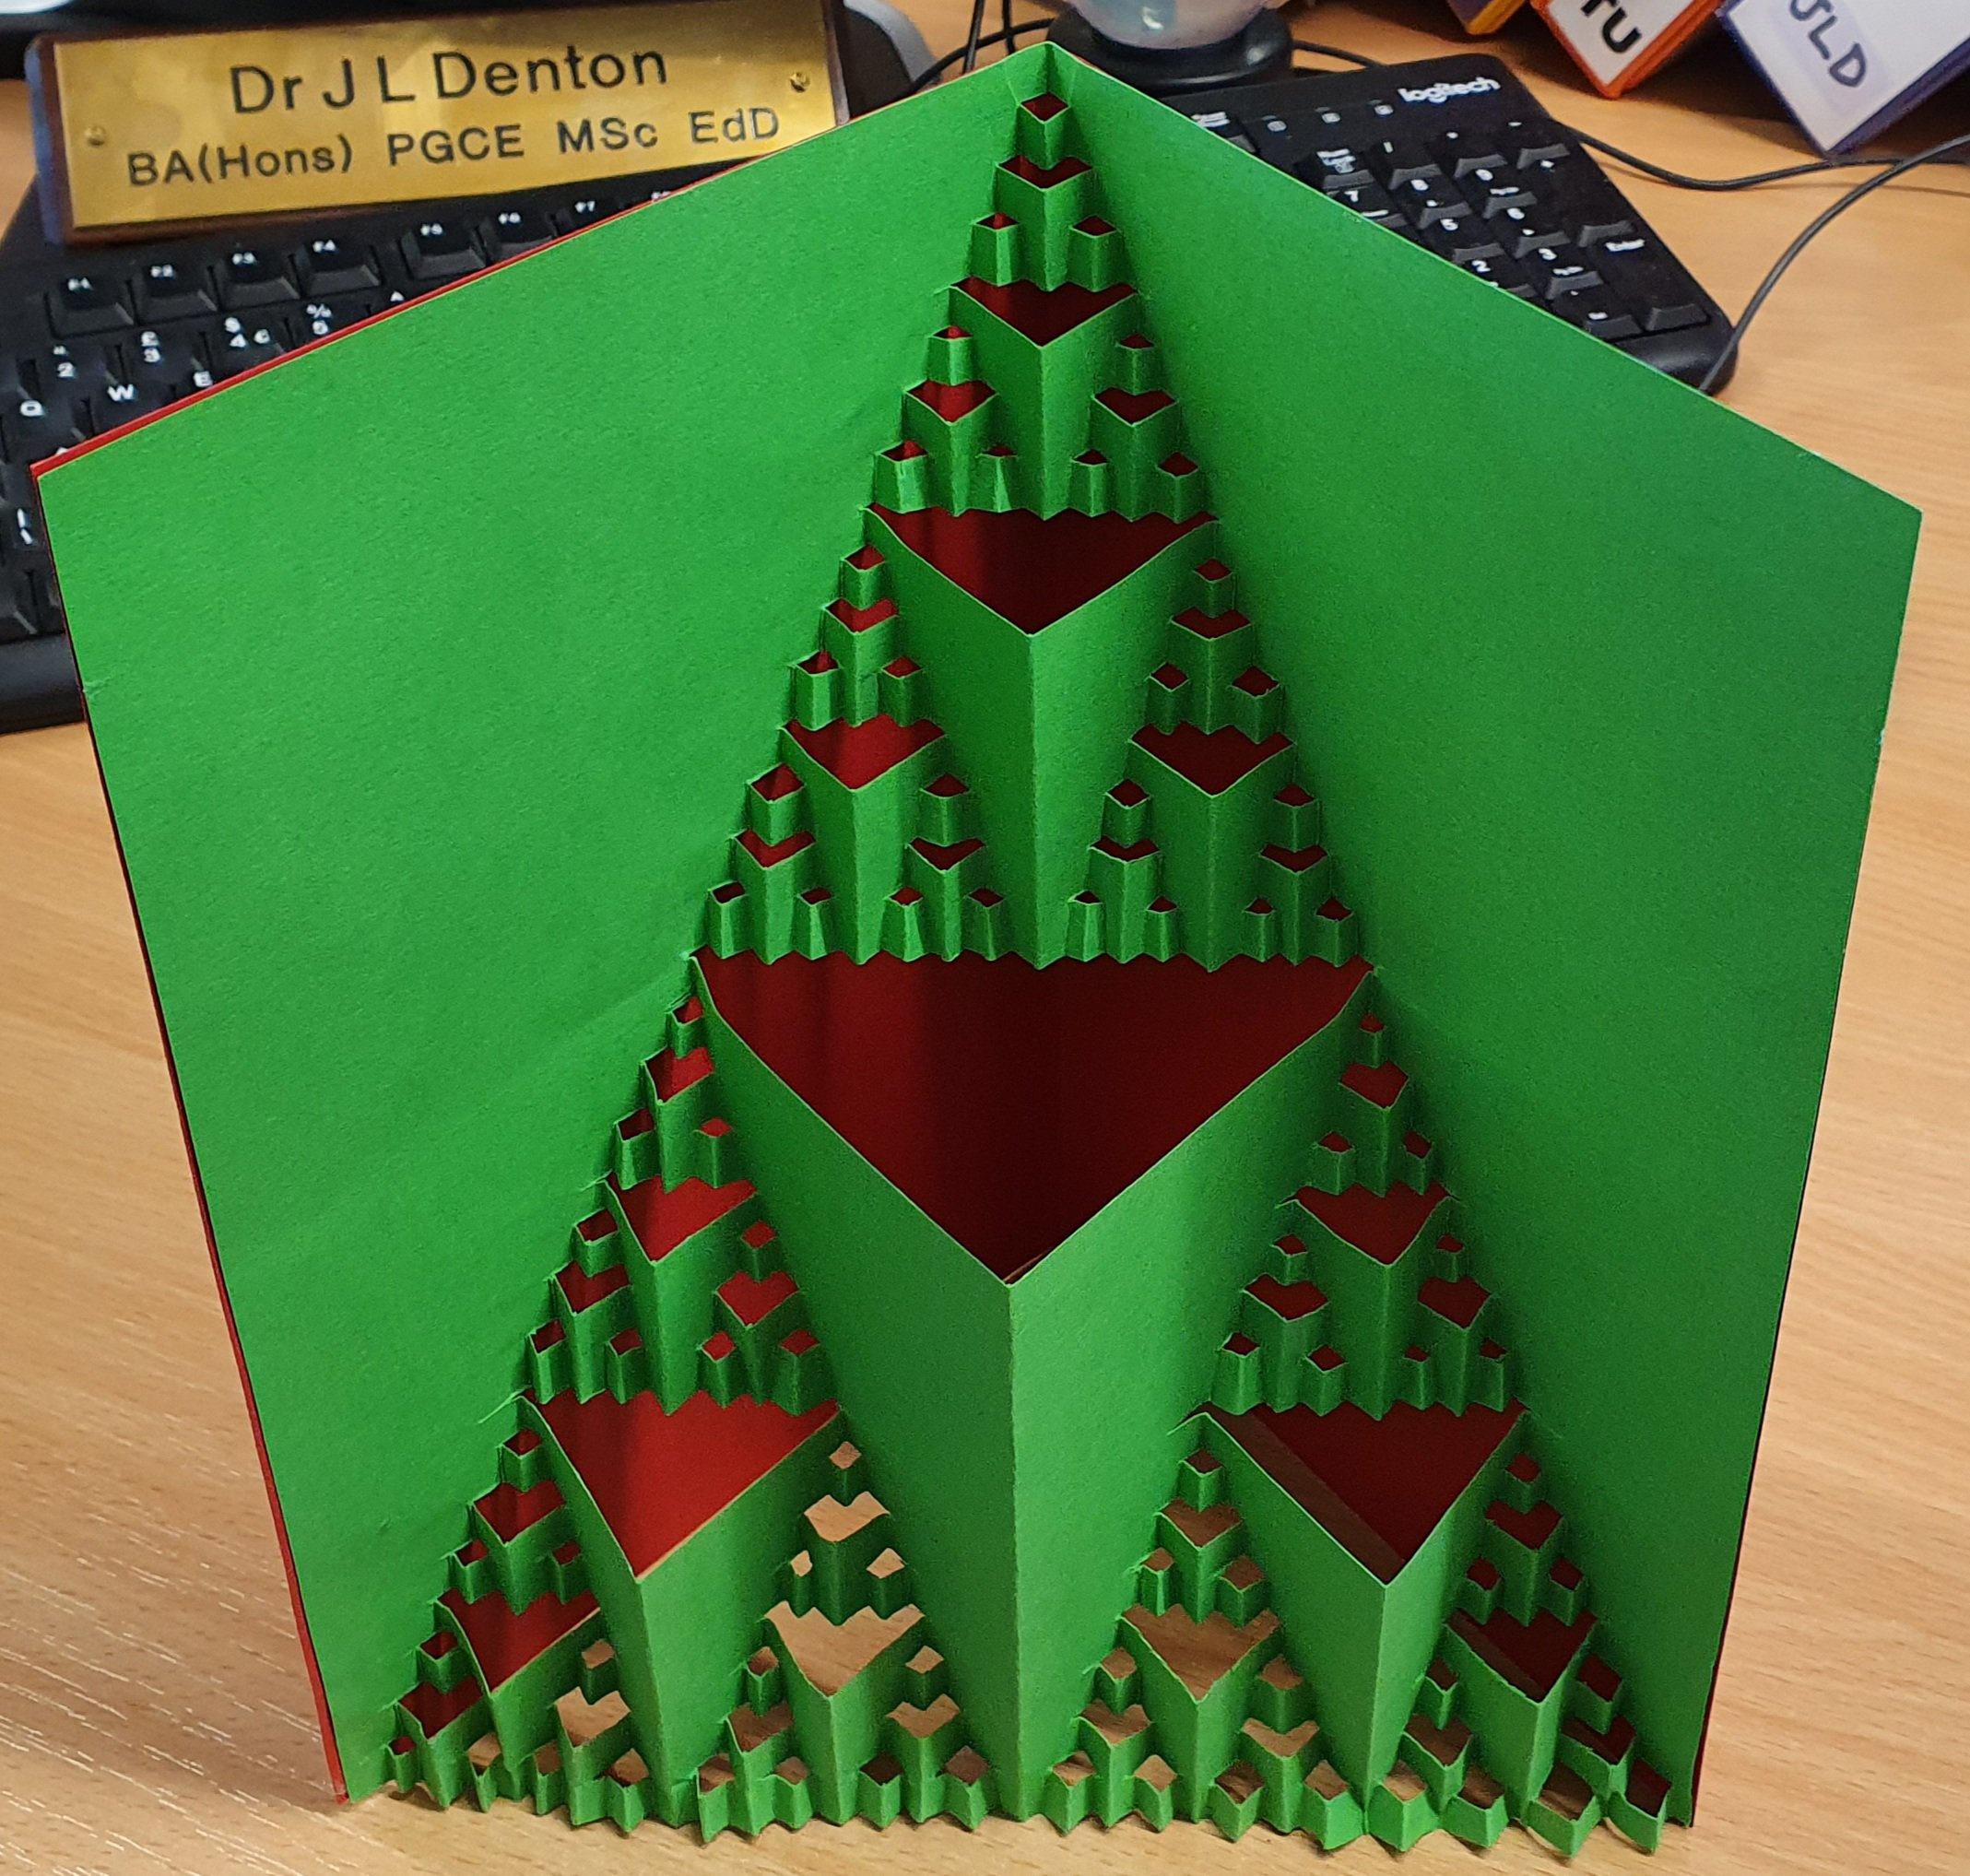
\includegraphics[width=0.5\textwidth]{figures/paper-sierspinsky-triangle.jpeg}
    \caption{Triángulo de Sierpinsky de papel.}
    \label{fig:paper-sierspinsky-triangle}
\end{figure}

\begin{figure}[H]
    \centering
    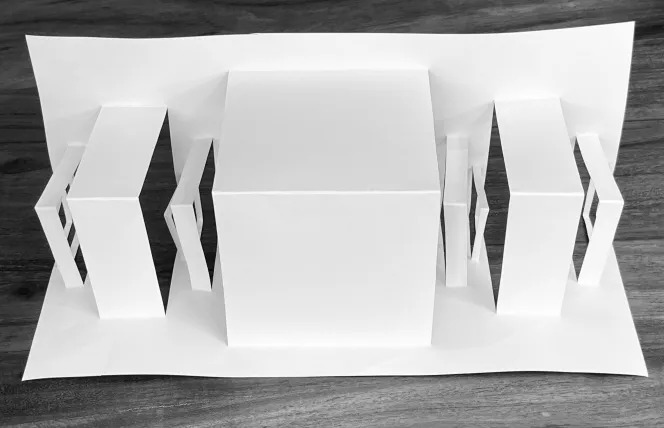
\includegraphics[width=0.5\textwidth]{figures/paper-cantor-set.jpg}
    \caption{Conjunto de Cantor de papel.}
    \label{fig:paper-cantor-set}
\end{figure}

\noindent Otros fractales los podemos hacer sin cortes, sinplementente con tiras de papel.\\

\begin{figure}[H]
    \centering
    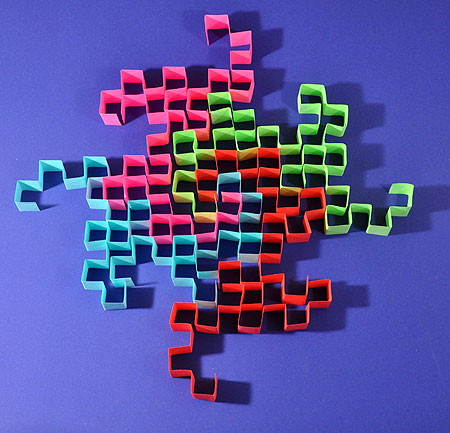
\includegraphics[width=0.5\textwidth]{figures/paper-dragon-curve.jpg}
    \caption{Curva de dragón de papel.}
    \label{fig:paper-dragon-curve}
\end{figure}